%
% Copyright (c) 2001 LAAS/CNRS                        --  Tue Oct 30 2001
% All rights reserved.                                     Anthony Mallet
%
% This document is a translation of the French documentation of GenoM,
% originally written by Sara Fleury and Matthieu Herrb.
%
% Redistribution  and  use in source   and binary forms,  with or without
% modification, are permitted provided that  the following conditions are
% met:
%
%   1. Redistributions  of  source code must  retain  the above copyright
%      notice, this list of conditions and the following disclaimer.
%   2. Redistributions in binary form must  reproduce the above copyright
%      notice,  this list of  conditions and  the following disclaimer in
%      the  documentation   and/or  other  materials   provided with  the
%      distribution.
%
% THIS SOFTWARE IS PROVIDED BY THE  AUTHOR AND CONTRIBUTORS ``AS IS'' AND
% ANY  EXPRESS OR IMPLIED WARRANTIES, INCLUDING,  BUT NOT LIMITED TO, THE
% IMPLIED WARRANTIES   OF MERCHANTABILITY AND  FITNESS  FOR  A PARTICULAR
% PURPOSE ARE DISCLAIMED.  IN NO  EVENT SHALL THE AUTHOR OR  CONTRIBUTORS
% BE LIABLE FOR ANY DIRECT, INDIRECT,  INCIDENTAL, SPECIAL, EXEMPLARY, OR
% CONSEQUENTIAL DAMAGES (INCLUDING,  BUT  NOT LIMITED TO, PROCUREMENT  OF
% SUBSTITUTE  GOODS OR SERVICES;  LOSS   OF  USE,  DATA, OR PROFITS;   OR
% BUSINESS  INTERRUPTION) HOWEVER CAUSED AND  ON ANY THEORY OF LIABILITY,
% WHETHER IN CONTRACT, STRICT LIABILITY, OR TORT (INCLUDING NEGLIGENCE OR
% OTHERWISE) ARISING IN ANY WAY OUT OF THE  USE OF THIS SOFTWARE, EVEN IF
% ADVISED OF THE POSSIBILITY OF SUCH DAMAGE.
%
% $Id$
%

This chapter will explain some vocabulary we use in this document, what
are modules, and how they work.

% -----------------------------------------------------------------------

\section{Vocabulary and general description}
\label{sec|module|voc}

A module lets  you integrate your  algorithms and functions  as  a set of
services in a  standard template. It then lets  you access those services
with a standardized  interface. Produced data can  also be retrieved in a
standard way.

The services are controlled (\emph{i.e.} parameterized, started or stopped)
with  \emph{requests},  that  represent  the    visible  part   of   the
module. Requests  will be sent by the operator using various interfaces
(\texttt{Test} program  generated   by /GenoM/ or  \texttt{tcl}  shell  - see 
paragraph~\vref{sec|tcl})    or  by a  program,    usually  named a  
\emph{supervisor},  that  will supervised  the  robot  (for  intance using 
\texttt{OpenPRS} - see paragraph~\vref{sec|propice}).
 
Each request can  have an \emph{input parameter} and an  
\emph{output parameter} (\texttt{C} structures as  of today). When a service ends,
a   \emph{reply} is sent to   the   client who invoked  the 
request. Each reply  is  associated with an  \emph{execution  report}:  it
reports on the execution of  the service and  lets  the client  know about
problems that might have occured.

There are two kind of requests: the \emph{execution} requests and the 
\emph{control} requests. Execution requests  start  an actual service,  whereas
control requests control the  execution of the services. Control requests
mainy allow to set parameters or  interrupt services. Each module has  a
predefined control request whose name  is  \texttt{Abort}: it can  interrupt
any running service as well as the module itself.

The execution time of  a control request  is considered to be zero. Thus,
they have only one final reply, which is  sent to the client immediately.
On the other hand, execution requests can last for an arbitrary amount of
time (even indefinitely). Thus they send an \emph{intermediate} reply,  as
soon as the service 
starts.  The final reply is sent when the service is over.

A running  service is called an   \emph{activity}. Some function,  such as
monitoring services,  can start \emph{several}  activities and  execute them
simultaneously. Other  kind   of function,  such as   servoing functions,
cannot handle  parallelism  and can only  start  \emph{one} activity at  a
time. This constraint has to be indicated by the developer.

Activities can control a physical device (sensors, actuators), read  data
produced by  other modules (by  the mean of  posters) or produce
data. These data can  be transfered at the end  of the  execution through
the final reply, or at any time by the mean of \emph{posters}.

A \emph{poster} is a structure (\texttt{C} and \texttt{XML} structure as  of  
today) that is
updated by an \texttt{activity} and shared in the global system. It can be read by
any other component of the system (a module, an operator, ...) at any time.

Every piece  of data that goes through  a module (requests or posters) is
stored  in an internal database  which is called \emph{Functional Internal
Data Structure} (fIDS  for short --- you might  also find the acronym
\emph{SDIf} which is the French translation of fIDS).

% -----------------------------------------------------------------------

\section{Structure and functioning of modules}
\label{sec|module|module}

As shown in the figure  \ref{fig|module}, a  module defines two  Internal
Data Structures:  the functional IDS (fIDS)  and  the control  IDS (cIDS)
dedicated to the internal routines.  The module also defines \emph{tasks}
(threads under Unix) that execute code. There are at least two tasks:

\begin{itemize}
\item One \emph{control task} that controls the module.
\item One (or several) \emph{execution tasks} that run your services and
the algorithms they are made of.
\end{itemize}

\begin{figure}[htbp]
\centering
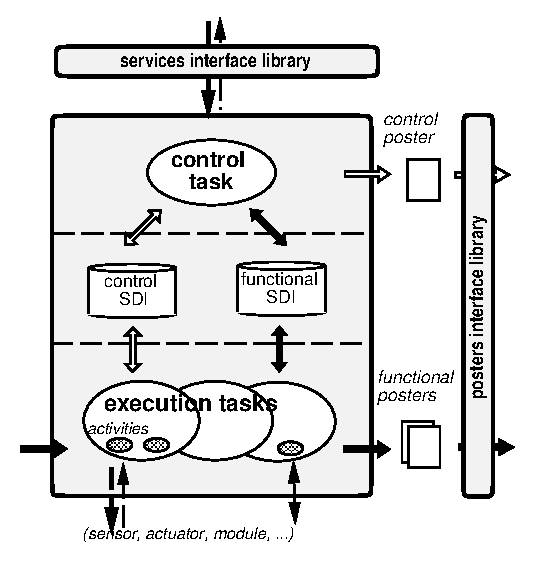
\includegraphics[width=0.5\hsize]{fig/module-en}
\caption{Structure of modules.}
\label{fig|module}
\end{figure}

\subsubsection{The control task:}

You normally do not have to care about the control task, but it's a good
idea to learn what it does. The control task

\begin{enumerate}
\item it receives the requests for the module,
\item it checks the validity of the input parameters and store them in the fIDS,
\item it checks if the module can start a given service (handles conflicts
between requests),
\item it tells the right execution task to start the service,
\item and upon the termination of a service it sends back to the client
any output produced by the service (the execution report and possibly the
C structure declared for that service).
\end{enumerate}

Beside    this, the control task  maintains   a poster  (the \emph{control
poster}) that contains informations on   the current state of the  module
(running services, activities, and so on).

Conflicts between services are   handled  according to the following  rule:  if
incompatible  services are to  be run  at the  same  time, \textbf{the last
request   has  the  priority}. Activities    that  happen to  be
incompatible  with that new request are  interrupted. This strategy matches a
\emph{reactivity} criterion and is systematically applied.

You must  declare  yourself which  services  are incompatible with  which
services. Note that   a service is  \emph{very often}  incompatible  with
itself; you must not forget to declare this.


\subsubsection{Execution tasks:}

Your own code is executed by the execution(s) task(s).

If  this code is to  be periodical (servoing,  monitoring, filters, ...),
you will have to use a periodical  execution task and specify its period.
It   is  also  possible   to use   a-periodical  tasks  and  a  sequential
scheduling. Tasks are  given priorities (supported under real-time
operating systems only),
depending on their constrains in terms of resources and CPU requirements.

In the  \texttt{demo} example,  there were  only one  execution  task 
(\texttt{exec\_task MotionTask}). 
This   is  usually  sufficient since  a   single
execution task can handle \emph{several}  activities in parallel. However,
if several  activities require different  priorities or periods, you will
have to declare several execution tasks.


\subsubsection{Interface libraries:}

Modules provide two standard interface libraries in various programming
languages (for now: \texttt{C, tcl, XML, open-prs}).

\begin{itemize}
\item A service library, which handles requests emission and reception,
\item A poster library, which contains the necessary functions to read
the module posters.
\end{itemize}


% -----------------------------------------------------------------------

\section{Integration of the algorithms: the codels}
\label{sec|module|codels}

In order to associate your code to the requests, you have to tell \GenoM\
which are the  functions that must be  executed to  handle requests. Your
algorithms must be split into several parts (startup, main function, end,
interruption, ...).   Each  of  these   parts  is called  a   \emph{codel}
(elementary code). At this time, codels are \texttt{C} functions.

A module is the result of  the link edition between  the code \GenoM\ has
generated and the codels libraries.
